
\section{Introduction}

A regex is a syntax used to define a pattern
that can then be matched against strings for
validation or data extraction.

To represent a regex $r$, one usually uses its
non-deterministic finite automaton (NFA)
\cite{thompson_programming_1968}, computed in $O(|r|)$
time complexity and which has $O(|r|)$ nodes.

\input{chapters/1-introduction/sample-nfas.tex}

We say that an $\epsilon$ transition (or a free move)
is an edge that does not consume a character.

\subsection*{Capturing Groups}

In the context of a regex, a capturing group $(X)$ can be used for the
extraction of subpatterns in a string. For example, one could use the regex
$\texttt{(\textbackslash d\{4\})-(\textbackslash d\{2\})-(\textbackslash d\{2\})}$
to extract the year, month and day from a date in YYYY-MM-DD format.

To account for this, some special nodes are added to the NFA that
perform an action when visited, such as tracking the current string
position. For example, the node $\#1:entry$ keeps track of the index
of the string at which it entered the group $1$.

\begin{center}
    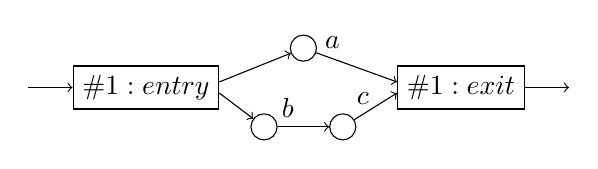
\begin{tikzpicture}
        \node[draw] (entry) at (-0.5, 0) {$\#1:entry$};
        \node[draw, circle] (up_a) at (1.5, 0.5) {};
        \node[draw, circle] (dw_b) at (1, -0.5) {};
        \node[draw, circle] (dw_c) at (2, -0.5) {};
        \node[draw] (exit) at (3.5, 0) {$\#1:exit$};

        \draw[->] ([xshift=-16]entry.west) -- (entry);
        \draw[->] ([yshift= 2pt]entry.east) -- (up_a);
        \draw[->] ([yshift=-2pt]entry.east) -- (dw_b);
        \draw[->] (dw_b) -- node[pos=0.2, above] (b) {$b$} (dw_c);
        \draw[->] (up_a) -- node[pos=0.2, above] (a) {$a$} ([yshift= 2pt]exit.west);
        \draw[->] (dw_c) -- node[pos=0.2, above] (c) {$c$} ([yshift=-2pt]exit.west);
        \draw[->] (exit) -- ([xshift=16]exit.east);
    \end{tikzpicture} \\ \vspace{0.3ex}
    \textit{NFA construction for $(a|bc)$}
\end{center}

The previous paper from the lab \cite{systemf_linear_2024} presented
a way to maintain capturing groups in $O(|r||s|)$ time and space complexity
as opposed to the state of the art $O(|r|^2|s|)$ time and $O(|r|^2)$ space
complexity.

The solution involved maintaining a set of linked lists, which shared many
redundant informations. This project presents a way to exploit this redundant 
information using Virtual Trees \cite{spike1236_virtual_2025} to reach an
$O(|r||s|)$ time complexity and $O(|r|^2)$ space complexity (See Section
\ref{sec:capture-groups-optimization-virtual-tree}).

\subsection*{Lookarounds}

Another feature that this project focuses on is lookarounds. It allows
the regex to search for a subpattern before or after the current
string position without consuming the characters.

For example, the regex \texttt{b(?=a)} will search for the letter $b$
followed by the letter $a$, without including the letter $a$ in the match.

The previous paper from the lab \cite{systemf_linear_2024} presented a way
to include that feature in the NFA by creating a lookup table for every
lookaround, known as its boolean oracle. This table contains one boolean per
potential starting position, whether the lookaround succeeds.


\begin{center}
    \begin{tikzpicture}
        \node[draw, circle] (nodeb) at (0, 0) {};
        \node[draw, inner sep=0.5, align=center] (nodea) at (3.5, 0) {
            \begin{tikzpicture}
                \node[draw, circle, inner sep=3.33pt] (root) at (0, 0) {};
                \draw[->] ([xshift=-16pt]root.west) -- (root);
                \draw[->] (root) -- node[pos=0.2, inner sep=3.33pt, above] (a) {$a$} ([xshift=16pt]root.east);
                \node (space) at (0, -0.4) {};
            \end{tikzpicture} \\

            \begin{tabular}{c|c|c|c|c|c}
                \hline
                Index & 0 & 1 & 2 & 3 & 4 \\ \hline
                Succeeds & \cmark & \xmark & \cmark & \xmark & \xmark \\
            \end{tabular}
        };

        \draw[->] ([xshift=-16pt]nodeb.west) -- (nodeb);
        \draw[->] (nodeb) -- node[pos=0.2, above] (b) {$b$} (nodea);
        \draw[->] (nodea) -- ([xshift=16pt]nodea.east);
    \end{tikzpicture} \\ \vspace{0.3ex}
    \textit{NFA construction for \texttt{b(?=a)} against string \texttt{abac}} \\
    \textit{The Lookaround succeeds if the character at that index is an }\texttt{a}
\end{center}


The computation and storage of these tables requires a time complexity of $O(|r||s|)$
and a space complexity of $O(|r||s|)$. My project focused on creating a new algorithm
that has a smaller space complexity of $O(|r| \sqrt{|s|})$ in exchange for a time
complexity of $O(|r||s| D)$, where $D$ is the maximum number of nested lookarounds
(See Section \ref{sec:memory-optimization-oracle}).

\subsection*{Atomic Groups}

In the context of a regex, an edge has a higher priority than another
edge going out of the same node if it is explored first by the backtracking engine.
A match is of higher priority than another match if it is found before
the other by the backtracking engine. For example, in $e_1|e_2$, $e_1$ has a higher
priority than $e_2$. For the greedy quantifier $e^*$, the engine prioritizes
matching the subpattern $e$ as many times as possible before continuing to the next
part of the pattern.

\begin{center}
    \begin{tabular}{c c}
        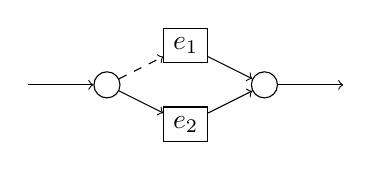
\begin{tikzpicture}
            \node[circle, draw] (start) at (0, 0) {};
            \node[draw] (e1) at (1, 0.5) {$e_1$};
            \node[draw] (e2) at (1, -0.5) {$e_2$};
            \node[circle, draw] (end) at (2, 0) {};
            
            \draw[->] (-1, 0) -- (start);
            \draw[->, dashed] (start) -- (e1); \draw[->] (e1) -- (end);
            \draw[->] (start) -- (e2); \draw[->] (e2) -- (end);
            \draw[->] (end) -- (3, 0);
        \end{tikzpicture} & 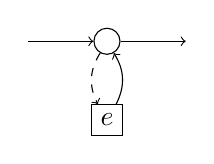
\begin{tikzpicture}
            \node[draw] (e) at (0, 0) {$e$};
            \node[draw, circle] (root) at (0, 1) {};
            
            \draw[->] (-1, 1) -- (root);
            \draw[->] (root) -- (1, 1);
            \draw[->, dashed] (root) to[bend right] (e);
            \draw[->] (e) to[bend right] (root);
        \end{tikzpicture}
    \end{tabular} \\ \vspace{0.3ex}
    \textit{NFA constructions for $e_1 \ | \ e_2$ and $e^*$} \\
    \textit{Dashed edges are higher priority edges.}
\end{center}

To avoid the exponential time of backtracking algorithms, many semantics provide
a special feature known as Atomic Groups. An Atomic Group is a group \texttt{(?>X)} that
only matches the highest priority match and discards all other matches.

For example, if we take the regex \texttt{(?>(b*|.))b} and try to match \texttt{bb},
it won't find any match as the atomic group will consume all the b's, leaving none
for the last character of the pattern. On the other hand, if we try to match \texttt{cb},
then it will succeed and the match will be the entire string.

It was shown that Atomic Groups may be used for Memoized Backtracking Engines
\cite{weirich_efficient_2024} in the case of NFA that do not have $\epsilon$
loops. This paper also states that the algorithm can easily be adapted to
both ECMAScript and Rust Semantics. During this project, we expressed doubts
regarding the existence of the second adaptation (at least for the stated time and
space complexity) and propose an example where we believe the adaptation
isn't as direct as stated (See Section \ref{sec:lookarounds-example}).

Using some of the tools described in the paper, this project presents
a new algorithm to adapt atomic groups for the PikeVM in ECMAScript Semantics
in $O(|r| |s|)$ time and $O(|r| |s|)$ space using a new oracle that
enforces that the thread follows the path towards its highest priority
match (See Section \ref{sec:lookarounds-linear-time-ecmascript}).

This project also conjectures that it should be possible in $\tilde{O}(|r||s|)$
time and $\tilde{O}(|r||s|)$ space to do the same technique for the
Rust Semantics using new tools such as Dominator Trees (See Section
\ref{sec:lookarounds-dominator-tree-conjecture}).

\subsection*{NFA Simulation and PikeVM}

More recent regexes engine, such as the PikeVM that we study in this project,
use an algorithm known as NFA Simulation. Instead of choosing one path in
the NFA and backtracking if it ends up failing to find a match, this algorithm
tracks every possible valid state of the NFA at the same time
\cite{thompson_programming_1968} \cite{russ_regular_2009}.

When the algorithm reads a character, it takes the list of active states,
known as threads and first applies all possible free moves before
consuming the character for all active threads.
\begin{center}
    \begin{tabular}{c c c}
        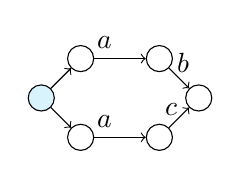
\begin{tikzpicture}
            \node[draw, circle, fill=cyan!15] (root)  at (0, 0) {};
            \node[draw, circle] (up1)   at (0.5, 0.5) {};
            \node[draw, circle] (down1) at (0.5, -0.5) {};
            \node[draw, circle] (up2)   at (1.5, 0.5) {};
            \node[draw, circle] (down2) at (1.5, -0.5) {};
            \node[draw, circle] (exit)  at (2, 0) {};

            \draw[->] (root) -- (up1);
            \draw[->] (root) -- (down1);
            \draw[->] (up1) -- node[pos=0.2, above] (a1) {$a$} (up2);
            \draw[->] (down1) -- node[pos=0.2, above] (a2) {$a$} (down2);
            \draw[->] (up2) -- node[pos=0.7, above] (b1) {$b$} (exit);
            \draw[->] (down2) -- node[pos=0.1, above] (c1) {$c$} (exit);
        \end{tikzpicture} & 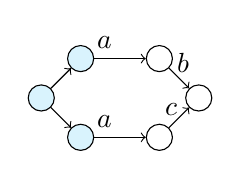
\begin{tikzpicture}
            \node[draw, circle, fill=cyan!15] (root)  at (0, 0) {};
            \node[draw, circle, fill=cyan!15] (up1)   at (0.5, 0.5) {};
            \node[draw, circle, fill=cyan!15] (down1) at (0.5, -0.5) {};
            \node[draw, circle] (up2)   at (1.5, 0.5) {};
            \node[draw, circle] (down2) at (1.5, -0.5) {};
            \node[draw, circle] (exit)  at (2, 0) {};

            \draw[->] (root) -- (up1);
            \draw[->] (root) -- (down1);
            \draw[->] (up1) -- node[pos=0.2, above] (a1) {$a$} (up2);
            \draw[->] (down1) -- node[pos=0.2, above] (a2) {$a$} (down2);
            \draw[->] (up2) -- node[pos=0.7, above] (b1) {$b$} (exit);
            \draw[->] (down2) -- node[pos=0.1, above] (c1) {$c$} (exit);
        \end{tikzpicture} & 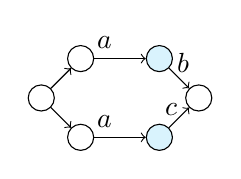
\begin{tikzpicture}
            \node[draw, circle] (root)  at (0, 0) {};
            \node[draw, circle] (up1)   at (0.5, 0.5) {};
            \node[draw, circle] (down1) at (0.5, -0.5) {};
            \node[draw, circle, fill=cyan!15] (up2)   at (1.5, 0.5) {};
            \node[draw, circle, fill=cyan!15] (down2) at (1.5, -0.5) {};
            \node[draw, circle] (exit)  at (2, 0) {};

            \draw[->] (root) -- (up1);
            \draw[->] (root) -- (down1);
            \draw[->] (up1) -- node[pos=0.2, above] (a1) {$a$} (up2);
            \draw[->] (down1) -- node[pos=0.2, above] (a2) {$a$} (down2);
            \draw[->] (up2) -- node[pos=0.7, above] (b1) {$b$} (exit);
            \draw[->] (down2) -- node[pos=0.1, above] (c1) {$c$} (exit);
        \end{tikzpicture} \\
        \textit{Initial Threads} & \textit{Free moves} & \textit{Consuming 'a'}
    \end{tabular}
    \begin{tabular}{c c}
        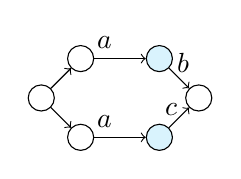
\begin{tikzpicture}
            \node[draw, circle] (root)  at (0, 0) {};
            \node[draw, circle] (up1)   at (0.5, 0.5) {};
            \node[draw, circle] (down1) at (0.5, -0.5) {};
            \node[draw, circle, fill=cyan!15] (up2)   at (1.5, 0.5) {};
            \node[draw, circle, fill=cyan!15] (down2) at (1.5, -0.5) {};
            \node[draw, circle] (exit)  at (2, 0) {};

            \draw[->] (root) -- (up1);
            \draw[->] (root) -- (down1);
            \draw[->] (up1) -- node[pos=0.2, above] (a1) {$a$} (up2);
            \draw[->] (down1) -- node[pos=0.2, above] (a2) {$a$} (down2);
            \draw[->] (up2) -- node[pos=0.7, above] (b1) {$b$} (exit);
            \draw[->] (down2) -- node[pos=0.1, above] (c1) {$c$} (exit);
        \end{tikzpicture} & 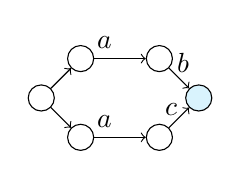
\begin{tikzpicture}
            \node[draw, circle] (root)  at (0, 0) {};
            \node[draw, circle] (up1)   at (0.5, 0.5) {};
            \node[draw, circle] (down1) at (0.5, -0.5) {};
            \node[draw, circle] (up2)   at (1.5, 0.5) {};
            \node[draw, circle] (down2) at (1.5, -0.5) {};
            \node[draw, circle, fill=cyan!15] (exit)  at (2, 0) {};

            \draw[->] (root) -- (up1);
            \draw[->] (root) -- (down1);
            \draw[->] (up1) -- node[pos=0.2, above] (a1) {$a$} (up2);
            \draw[->] (down1) -- node[pos=0.2, above] (a2) {$a$} (down2);
            \draw[->] (up2) -- node[pos=0.7, above] (b1) {$b$} (exit);
            \draw[->] (down2) -- node[pos=0.1, above] (c1) {$c$} (exit);
        \end{tikzpicture} \\
        \textit{Free moves} & \textit{Consuming 'b'}
    \end{tabular} \\ \vspace{0.3ex}
    \textit{Example of NFA simulation for the string "ab"} \\
    \textit{Cyan represents threads, and red means the edge was used during that step.}
\end{center}

In particular, since the NFA is of size $O(|r|)$, there are only $O(|r|)$
active threads at any point in time (you don't maintain two threads that are
on the same node at the same time as they have the same future, and so only
the highest priority thread matters).

To make the regex matching fast, the PikeVM algorithm treats the regex
as a program, turning the NFA into bytecode, where each instruction tells
the engine how to continue matching from the state.

\begin{center}
    \begin{tikzpicture}
        \node[draw, circle] (root)  at (0, 0) {\texttt{0}};
        \node[draw, circle] (up1)   at (1, 0.5) {\texttt{1}};
        \node[draw, circle] (down1) at (1, -0.5) {\texttt{3}};
        \node[draw, circle] (up2)   at (2, 0.5) {\texttt{2}};
        \node[draw, circle] (down2) at (2, -0.5) {\texttt{4}};
        \node[draw, circle, accepting] (exit)  at (3, 0) {\texttt{5}};

        \draw[->] (root) -- (up1);
        \draw[->] (root) -- (down1);
        \draw[->] (up1) -- node[pos=0.2, above] (a1) {$a$} (up2);
        \draw[->] (down1) -- node[pos=0.2, above] (a2) {$a$} (down2);
        \draw[->] (up2) -- node[pos=0.7, above] (b1) {$b$} (exit);
        \draw[->] (down2) -- node[pos=0.1, above] (c1) {$c$} (exit);
    \end{tikzpicture} \\ \vspace{1ex}
    \begin{tabular}{l l}
        \texttt{0:} & \texttt{FORK 1 3} \\
        \texttt{1:} & \texttt{CONSUME 2 \textnormal{a}} \\
        \texttt{2:} & \texttt{CONSUME 5 \textnormal{b}} \\
        \texttt{3:} & \texttt{CONSUME 4 \textnormal{a}} \\
        \texttt{4:} & \texttt{CONSUME 5 \textnormal{c}} \\
        \texttt{5:} & \texttt{ACCEPT}
    \end{tabular} \\ \vspace{0.3ex}
    \textit{Example bytecode for \textsc{(ab|ac)}}
\end{center}
